% This work is licensed under the Creative Commons
% Attribution-NonCommercial-ShareAlike 4.0 International License. To view a copy
% of this license, visit http://creativecommons.org/licenses/by-nc-sa/4.0/ or
% send a letter to Creative Commons, PO Box 1866, Mountain View, CA 94042, USA.

\chapter{Der Stetigkeitssatz von Lévy} %8
\textbf{Ziel:}
\begin{itemize}
	\item Das Beschreiben von Konvergenz in Verteilung mittels charakteristischer Funktion
	\item Wichtig für zentrale Grenzwertsätze
\end{itemize}

Zur Erinnerung:

\begin{defi}[Konvergenz in Verteilung]\enter
	Seien $(Y_n)_{n\in\N}$, $Y$ $\R^d$-wertige Zufallsvariablen.
	Wir sagen $(Y_n)_{n\in\N}$ \textbf{konvergiert in Verteilung} gegen $Y$, i. Z.
	\begin{align*}
		Y_n\overset{\d}{\longrightarrow}Y
		:\Longleftrightarrow\forall f\in C_b\big(\R^d\big):
		\E\big[f(Y_n)\big]\overset{n\to\infty}{\longrightarrow}\E\big[f(Y)\big]
	\end{align*}
\end{defi}

\begin{defi}[schwache Konvergenz]\enter
	Seien $(\mu_n)_{n\in\N},\mu\in\M_b\big(\R^d\big)$ beschränkte Borelmaße.
	Wir sagen $(\mu_n)_{n\in\N}$ \textbf{konvergiert schwach gegen} $\mu$, i.Z.
	\begin{align*}
		\mu_n\overset{\w}{\longrightarrow}\mu 
		:\Longleftrightarrow\forall f\in C_b\big(\R^d\big):\int\limits f\d\mu_n\overset{n\to\infty}{\longrightarrow}\int\limits f\d\mu 
	\end{align*}
\end{defi}

\begin{bemerkung}\
	\begin{itemize}
		\item Sei $\P_Y$ das von $Y$ \textbf{induzierte} Maß in $\M_b(\R^d)$, d.h.
		\begin{align*}
			\P_Y(B):=\P(Y\in B):=\P\big(\lbrace\omega\in\Omega:B(\omega)\in B\rbrace\big)\qquad\forall B\in\B\big(\R^d\big)
		\end{align*}
		Dann gilt:
		\begin{align}\label{eqBemerkungChapter8}\tag{$\ast$}
			\P_{Y_n}\overset{\w}{\longrightarrow}\P_Y
			\Longleftrightarrow
			Y_n\overset{\d}{\longrightarrow} Y
		\end{align}
		Also schwache Konvergenz der induzierten Maße ist äquivalent zur Konvergenz in Verteilung.
		\item In Dimension $d=1$ kann Konvergenz in Verteilung auch folgendermaßen formuliert werden:\nl
		Seien $(F_n)_{n\in\N}$ und $F$ die Verteilungsfunktionen von $(Y_n)_{n\in\N}$ und $Y$. 
		Dann gilt:
		\begin{align*}
			Y_n\overset{\d}{\longrightarrow}Y
			\Longleftrightarrow\forall\text{ Stetigkeitspunkte $x$ von }F:
			F_n(x)\overset{n\to\infty}{\longrightarrow} F(x)
		\end{align*}
	\end{itemize}
\end{bemerkung}

\begin{theorem}[Stetigkeitssatz von Lévy]\label{theorem8.1StetigkeitssatzVonLevy}\enter
	Seien $(\mu_n)_{n\in\N}\subseteq\M_b(\R^d)$ eine Folge von beschränkten Borelmaßen.
	\begin{enumerate}[label=(\alph*)]
		\item Wenn $\mu_n\overset{\w}{\longrightarrow}\mu$ für $\mu\in\M_b(\R^d)$, dann gilt
		\begin{align*}
			\hat{\mu}_n(\xi)\overset{n\to\infty}{\longrightarrow}\hat{\mu}(\xi)\qquad\forall\xi\in\R^d
		\end{align*}
		Also: Schwache Konvergenz der Maße bedeutet punktweise Konvergenz der Fouriertransformation.
		\item Wenn $\hat{\mu}_n(\xi)\overset{n\to\infty}{\longrightarrow}\phi(\xi)$ $\forall\xi\in\R^d$ und $\phi:\R^n\to\R$ ist stetig bei $\xi=0$, 
		dann existiert 
		\begin{align*}
			\mu\in\M_b(\R^d) \mit \mu_n\overset{\w}{\longrightarrow}\mu \text{ und } \phi=\hat{\mu}.
		\end{align*}
		Also: Punktweise Konvergenz der Fouriertransformation \underline{und} Grenzfunktion $\phi$ ist stetig in 0 $\implies$ schwache Konvergenz der Maße.
	\end{enumerate}
\end{theorem}

Mit Äquivalenz \eqref{eqBemerkungChapter8} zu schwacher Konvergenz und Konvergenz in Verteilung erhalten wir:

\begin{korollar}\label{korollar8.2}
	Sei $(Y_n)_{n\in\N}$ ein Folge von $\R^d$-wertigen Zufallsvariablen.
	\begin{enumerate}[label=(\alph*)]
		\item $\begin{aligned}
			Y_n\overset{\d}{\longrightarrow} Y\implies\forall\xi\in\R^d:\Phi_{Y_n}(\xi)\overset{n\to\infty}{\longrightarrow}\Phi_Y(\xi)
		\end{aligned}$
		\item Wenn $\begin{aligned}
			 \Phi_{Y_n}(\xi)\overset{n\to\infty}{\longrightarrow}\phi(\xi)~\forall\xi\in\R^d
		\end{aligned}$
		\underline{und} $\phi$ ist stetig bei $\xi=0$, dann existiert eine Zufallsvariable $Y$ mit $Y_n\overset{\d}{\longrightarrow}Y$ und $\Phi_Y=\phi$.
	\end{enumerate}
\end{korollar}

\begin{bemerkung}\
	\begin{itemize}
		\item Die Konvergenz in (a) ist \textbf{gleichmäßig auf Kompakta}, d.h.
		\begin{align*}
			\sup\limits_{|\xi|\leq R}\Big|\mu_n(\xi)-\mu(\xi)\Big|\overset{n\to\infty}{\longrightarrow}0
		\end{align*}
		\item Der Grenzwert $\mu$ (bzw. $Y$) ist eindeutig 
		(Folgt aus Eindeutigkeitssatz für Fouriertransformation bzw. charakteristische Funktionen, Theorem \ref{theorem7.6Eindeutigkeitssatz}).
	\end{itemize}
\end{bemerkung}

\begin{proof}[Beweis des Stetigkeitssatzes von Lévy \ref{theorem8.1StetigkeitssatzVonLevy}, Teil (a)]\enter
	Für $\xi\in\R^d$ setze
	\begin{align*}
		f_\xi(x):=\exp\big(i\cdot x^T\cdot\xi\big).
	\end{align*}
	Dies ist offenbar eine stetige und beschränkte Funktion, also $f_\xi\in C_b(\R^d)$.
	Also gilt
	\begin{align*}
		\hat{\mu}_n(\xi)
		&=\int\limits_{\R^d}\exp\big(i\cdot x^T\cdot\xi\big)~\mu_n(\d x) \\
		&=\int\limits_{\R^d} \underbrace{f_\xi}_{\in C_b(\R^d)}\d\mu_n \\
		&\overset{\text{w}}{\longrightarrow}
		\int\limits_{\R^d}f_\xi\d\mu\\
		&=\int\limits_{\R^d}\exp\big(i\cdot x^T\cdot\xi\big)~\mu(\d x) \\
		&=\hat{\mu}(\xi)
		\qquad\forall\xi\in\R^d
	\end{align*}
\end{proof}

\begin{beisp}[Normalapproximation der Binomialverteilung]\enter
	Sei $(X_n)_{n\in\N}\sim\Bin(n,p)$ und $p\in(0,1),q:=1-p$. Setze
	\begin{align*}
		Y_n:
		&=\frac{X_n-\E[X_n]}{\sqrt{\Var(X_n)}}
		=\frac{X_n-n\cdot p}{\sqrt{n\cdot p\cdot q}}
		=\frac{X_n}{\sqrt{n\cdot p\cdot q}}-\sqrt{\frac{n\cdot p}{q}}
	\end{align*}
	Charakteristische Funktion der Binomialverteilung(siehe Tabelle und Übung):
	\begin{align*}
		\Phi_{X_n}(u)
		&=\Big(1+p\cdot\big(\exp(i\cdot u)-1\big)\Big)^n\\
		\Phi_{Y_n}(u)
		&=\exp\left(-i\cdot u\cdot\sqrt{\frac{n\cdot p}{q}}\right)\cdot\Phi_{X_n}\left(\frac{u}{\sqrt{n\cdot p\cdot q}}\right)
	\end{align*}
	Logarithmieren:
	\begin{align*}
		\log\big(\Phi_{Y_n}(u)\big)
		&=-i\cdot u\cdot\sqrt{\frac{n\cdot p}{q}}+n\cdot\log\left(1+p\cdot\left(\exp\left(\frac{i\cdot u}{\sqrt{n\cdot p\cdot q}}\right)-1\right)\right) 
	\end{align*}
	Grenzübergang $n\to\infty$: Nutze Taylorentwicklung der Exponentialfunktion:
	\begin{align*}
		\exp(x)
		&=1+x+\frac{x^2}{2}+\O\big(x^3\big)\\
		\log(1+x)
		&=x-\frac{x^2}{2}+\O\big(x^3\big)\\
		%\implies
		\log\big(\Phi_{Y_n}(u)\big)
		&=-i\cdot u\cdot\sqrt{\frac{n\cdot p}{q}}+n\cdot\log\left(1+i\cdot u\cdot\sqrt{\frac{p}{n\cdot q}}-\frac{u^2}{2}\cdot\frac{1}{n\cdot q}+\O\left(n^{-\frac{3}{2}}\right)\right)\\
		&=-i\cdot u\cdot\sqrt{\frac{n\cdot p}{q}}+n\cdot\left(i\cdot u\cdot\sqrt{\frac{p}{n\cdot q}}-\frac{u^2}{2}\cdot\frac{1}{n\cdot q}+\frac{u^2}{2}\cdot\frac{p}{n\cdot q}+\O\left(n^{-\frac{3}{2}}\right)\right)\\
		&=\sqrt{n}\cdot i\cdot u\cdot\underbrace{\left(\sqrt{\frac{p}{q}}-\sqrt{\frac{p}{q}}\right)}_{=0}-\frac{u^2}{2}\cdot\underbrace{\left(\frac{1}{q}-\frac{p}{q}\right)}_{=1}+\O\left(n^{-\frac{1}{2}}\right)
		\overset{n\to\infty}{\longrightarrow}-\frac{u^2}{2}\\
		&\implies
		\limn\Phi_{Y_n}(u)=\exp\left(-\frac{u^2}{2}\right)
	\end{align*}
	Da $u\mapsto\exp\left(-\frac{u^2}{2}\right)$ offenbar stetig in $u=0$ und charakteristische Funktion von $\Nor(0,1)$ ist, 
	folgt aus dem Stetigkeitssatz von Lévy \ref{theorem8.1StetigkeitssatzVonLevy}:
	\begin{align*}
		\exists\text{ Zufallsvariable }Y\sim\Nor(0,1)\mit Y_n\overset{\d}{\longrightarrow}Y.
	\end{align*}
\end{beisp}

Noch zu zeigen: Theorem \ref{theorem8.1StetigkeitssatzVonLevy} (b). 
Wir benötigen dafür (ohne Beweis):

%\setcounter{satz}{1} %Notwendig, da Prof so nummerierte (er hat Korollar 8.2 auf Wunsch eingeschoben)
\begin{lemma}\label{lemma8.2}
	$C_c^\infty(\R^d)$ (Testfunktionen) ist dicht in $C_\infty(\R^d)$ (stetige Funktionen, die bei Unendlich verschwinden) bzgl. $\Vert\cdot\Vert_\infty$.\\
	Intuition: %TODO Add Sketch
	% Das hier ist der Sketch aus der VL. Ich würde ihn aber rauslassen, da er (glaube ich) nicht richtig ist. Die Grenzfunktion mit der Spitze kann nicht in C_infty sein, da sie im Punkt der Spitze nicht unendlich glatt ist.
	% \begin{figure}[ht!]
	% 	\begin{center}
	% 		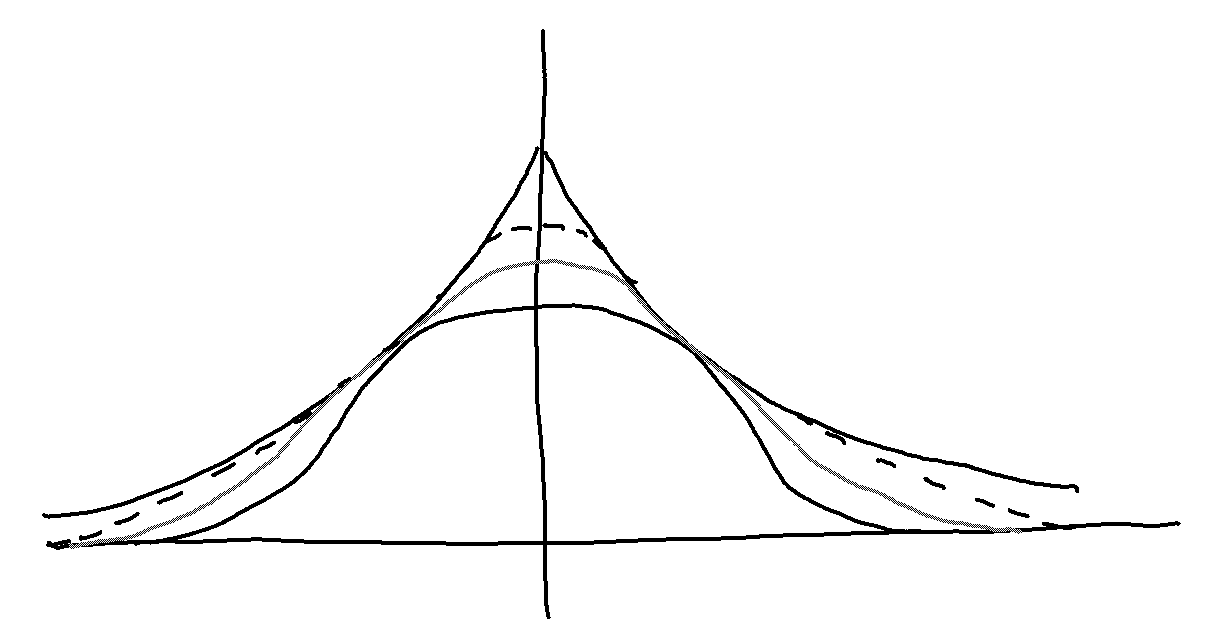
\includegraphics[width=0.75\textwidth]{./pics/Sketch4.png}
	% 		\caption{Funktionenfolge aus $C^\infty_c$, die gegen Funktion in $C^\infty$ konvergiert}
	% 		\label{AbbTestfunktionenDicht}
	% 	\end{center}
	% \end{figure}
\end{lemma}

\begin{theorem}[Rieszscher Darstellungssatz für $\M_b(\R^d)$]\label{theorem8.4RieszscherDarstellungssatzFuerM_b}\enter
	Sei $\Lambda:C_\infty(\R^d)\to\R$ ein lineares, positives, stetiges Funktional, d.h.
	\begin{itemize}
		\item $\begin{aligned}
			\Lambda(\alpha\cdot f+g)=\alpha\cdot\Lambda(f)+\Lambda(g)\qquad\forall\alpha\in\R,\forall f,g\in C_\infty
		\end{aligned}$ (Linearität)
		\item $\begin{aligned}
			f\geq0\implies\Lambda(f)\geq0
		\end{aligned}$ (Positivität)
		\item $\begin{aligned}
			\big|\Lambda(f)\big|\leq C_\Lambda\cdot\Vert f\Vert_\infty\qquad\forall f\in C_\infty
		\end{aligned}$ (beschränkt + linear $\implies$ stetig)
	\end{itemize} 
	Dann existiert ein \underline{eindeutiges} $\mu\in\M_b(\R^d)$ so, dass $\Lambda$ wird durch $\mu$ \textbf{dargestellt} wird, d.h.
	\begin{align*}
		\Lambda(f)=\int\limits f\d\mu\qquad\forall f\in C_\infty(\R^d)
	\end{align*}
	Also ist $\M_b(\R^d)$ der Dualraum (im Sinne der Funktionalanalysis) von $C_\infty(\R^d)$.
\end{theorem}

Folgende Definition aus der Maßtheorie wird noch benötigt:

\begin{defi}[Straffheit]
	Eine Folge $(\mu_n)_{n\in\N}\subseteq\M_b(\R^d)$ heißt \textbf{straff}
	\begin{align*}
		:\Longleftrightarrow
		\forall\varepsilon>0:\exists K_\varepsilon\subseteq\R^d\text{ kompakt},\exists N_\varepsilon\in\N:\forall n\geq N_\varepsilon:
		\mu_n\big(\R^d\setminus K_\varepsilon\big)\leq\varepsilon
	\end{align*}
\end{defi}

\begin{bemerkung}\
	\begin{itemize}
		\item Intuition: Bei straffer Folge "verschwindet" keine Masse nach Unendlich
		\item Jede straffe Folge enthält schwach konvergente Teilfolge.
		\item Beispiel für \underline{nicht}-straffe Folge: 
		\begin{align*}
			\mu_n(\d x):=\phi(x-n)\d x
			\quad\mit\quad
			\phi(x):=\frac{1}{\sqrt{2\cdot\pi}}\cdot\exp\left(-\frac{x^2}{2}\right)\text{
			(Dichte von $\Nor$)}
		\end{align*}

		\begin{figure}[ht!]
			\begin{center}
				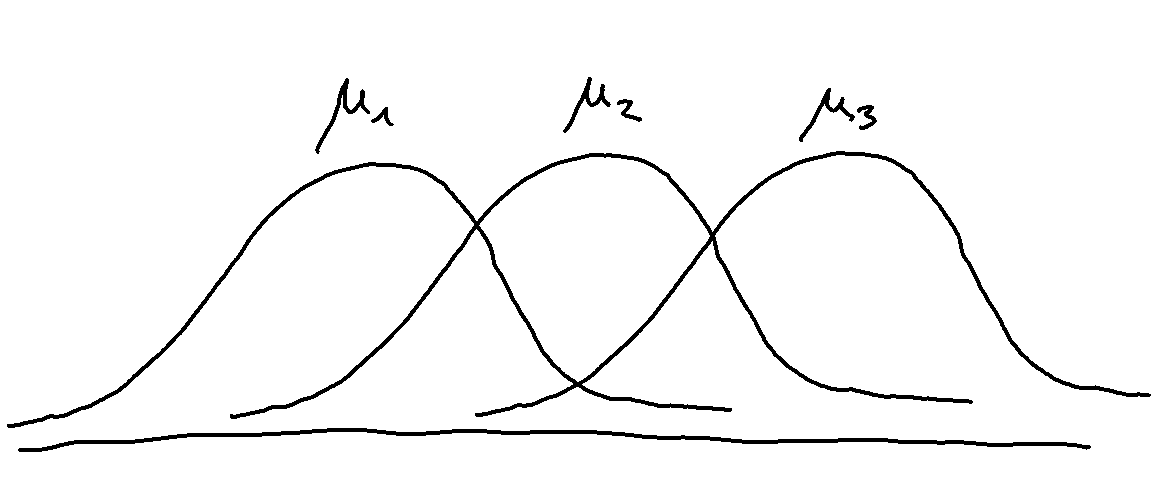
\includegraphics[width=0.75\textwidth]{./pics/Sketch5.png}
				\caption{Masse bewegt sich immer weiter}
				\label{AbbNichtStraffesMass}
			\end{center}
		\end{figure}
	\end{itemize}
\end{bemerkung}

Zusammenhang: Straffheit $\longleftrightarrow$ Fouriertransformation

\begin{lemma}\label{lemma8.5}
	Sei $\mu\in\M_b(\R)$.
	Dann gilt:
	\begin{align*}
		\mu\Big(\R\setminus[R,R]\Big)\leq
		c\cdot R\cdot\int\limits_0^{\frac{1}{R}}\Big(\hat{\mu}(0)-\Re\big(\hat{\mu}(\xi)\big)\Big)\d\xi
		\qquad\forall R>0\qquad
		\mit c=\frac{1}{1-\sin(1)}\leq 7
	\end{align*}
\end{lemma}

\begin{proof}
	Vorüberlegung: Betrachte Sinusfunktion:
		\begin{figure}[ht!]
			\begin{center}
				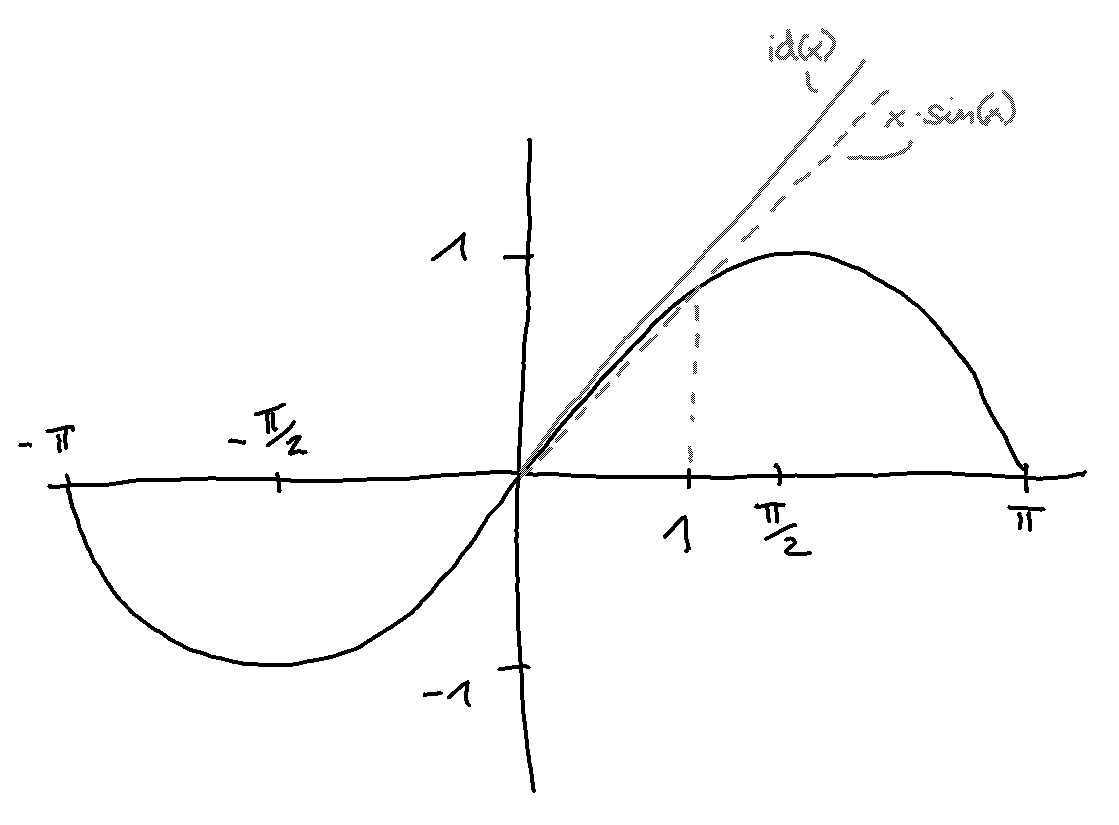
\includegraphics[width=0.75\textwidth]{./pics/Sketch6.png}
				\caption{Abschätzungen des Sinus}
				\label{AbbSinusAbschätzung}
			\end{center}
		\end{figure}
	\begin{align*}
		\left\lbrace
		\begin{array}{rl}
			\sin(x) \leq x & \forall x\geq 0 \\
			\sin(x) \geq x & \forall x\leq 0
		\end{array}\right. \implies
		\frac{\sin(x)}{x}\leq 1~\forall x\in\R \\
	\end{align*}
	und
	\begin{align*}
		\left\lbrace
		\begin{array}{rl}
			\sin(x) \leq x \cdot \sin(1) & \forall x\geq 0 \\
			\sin(x) \geq x \cdot \sin(1) & \forall x\leq 0
		\end{array}\right. \implies
		\frac{\sin(x)}{x}\leq\sin(1)~\forall x\in\R\setminus[-1,1]
	\end{align*}
	Also gilt:
	\begin{align*}
		R\cdot\int\limits_0^{\frac{1}{R}}\Big(\hat{\mu}(0)-\Re\big(\hat{\mu}(\xi)\big)\Big)\d\xi
		&=R\cdot\int\limits_0^{\frac{1}{R}}\left(\mu(\R)-\Re\left(\int\limits_{-\infty}^{\infty}\exp\big(i\cdot\xi\cdot x\big)~\mu(\d x)\right)\right)\d\xi\\
		&=R\cdot\int\limits_0^{\frac{1}{R}}\int\limits_{-\infty}^{\infty}\Big(1- \cos(x\cdot\xi)\Big)~\mu(\d x)\d\xi\\
		\overset{\text{Fub}}&=
		R\cdot\int\limits_{-\infty}^{\infty}\int\limits_0^{\frac{1}{R}}\big(1-\cos(x\cdot\xi)\big)\d\xi~\mu(\d x)\\
		&=R\cdot\int\limits_{-\infty}^{\infty}\left(\frac{1}{R}-\frac{\sin\left(\frac{x}{R}\right)}{x}\right)~\mu(\d x)\\
		&=\int\limits_{-\infty}^{\infty}\underbrace{\left(1-\frac{\sin\left(\frac{x}{R}\right)}{\frac{x}{R}}\right)}_{
		\begin{subarray}{c}		
			\geq0\\
			\geq1-\sin(1)\falls\left|\frac{x}{R}\right|\geq1\text{ bzw. }|x|\geq R
		\end{subarray}}~\mu(\d x)\\
		&\geq
		\big(1-\sin(1)\big)\cdot\mu\big(R\setminus[-R,R]\big)
	\end{align*}
\end{proof}

\begin{proof}[Beweis des Stetigkeitssatzes von Lévy \ref{theorem8.1StetigkeitssatzVonLevy}, Teil (b), nur für Dimension $d=1$]\enter
	\textbf{Teil 1: Kandidaten für Grenzwert $\mu$:}\\
	Wir wissen $\hat{\mu}_n(\xi)\overset{}{\longrightarrow}\phi(\xi)$.
	Wie können wir aus $\phi$ das Maß $\mu$ konstruieren?
	Betrachte $f\in S(\R)$ (Schwartz-Funktion).
	\begin{align}\label{eqProof8.1TeilBSTern}\tag{$\ast$}
		\int\limits f\d\mu_n
		\overset{\ref{korollar7.5SatzvonPlaucharel}}&=
		\int\limits\hut{f}(\xi)\hat{\mu}_n(\xi)\d\xi
		\overset{n\to\infty}{\longrightarrow}
		\underbrace{\int\limits\hut{f}(\xi)\phi(\xi)\d\xi}_{=:\Lambda(f)}
	\end{align}
	Behauptung: $\Lambda:S(\R)\to\R$ ist positives lineares stetiges Funktional.
	\begin{itemize}
		\item Linearität folgt aus der Fouriertransformation und Linearität des Integrals.
		\item Positivität (d.h. $f\geq0\implies\Lambda(f)\geq0$) gilt auch als Limes von positiven Funktionalen.
		\item Stetigkeit (bzw. Beschränktheit):
		\begin{align*}
			\big|\Lambda(f)\big|
			&=\left|\limn\int\limits f\d\mu_n\right| \\
			&\leq\Vert f\Vert_\infty\cdot\limn\mu(\R)\\
			&=\Vert f\Vert_\infty\cdot\limn\hat{\mu}_n(0)\\
			&=\Vert f\Vert_\infty\cdot\phi(0)
			<\infty
		\end{align*}
	\end{itemize}
	
	Da die Schwartz-Funktionen $S(\R)$ dicht in $\big(C_\infty(\R),\Vert\cdot\Vert_\infty\big)$ sind, 
	kann $\Lambda$ eindeutig auf $C_\infty(\R)$ fortgesetzt werden. 
	Auch \eqref{eqProof8.1TeilBSTern} setzt sich fort.\\
	Darstellungssatz von Riesz sagt nun: 
	Es existiert ein Maß $\mu\in\M_b(\R)$ mit
	\begin{align*}
		\int\limits\hut{f}(\xi)\phi(\xi)\d\xi
		&=\Lambda(f)
		=\int\limits f\d\mu\\
		\implies\limn\int\limits f\d\mu_n 
		&=\int\limits f\d\mu 
		\qquad\forall f\in C_\infty(\R)
	\end{align*}
	Wir brauchen diese Aussage aber alle $f$ aus $C_b(\R)$ statt $C_\infty(\R)$. 
	Hierfür brauchen wir die Straffheit.\nl
	\textbf{Teil 2: Straffheit der Folge}\\
	Es gilt:
	\begin{align}\nonumber
		\hat{\mu}_n(\xi)&\overset{n\to\infty}{\longrightarrow}\phi(\xi) &\forall\xi\in\R\\
		\implies\nonumber
		\underbrace{\Big(\hat{\mu}_n(0)-\Re\big(\hat{\mu}_n(\xi)\big)\Big)}_{|\cdot|\leq2}&\overset{n\to\infty}{\longrightarrow}\Big(\phi(0)-\Re\big(\phi(\xi)\big)\Big) &\forall\xi\in\R\\
		\overset{\text{dom Konv}}{\implies}\label{eqProof8.1TeilBPlus}\tag{+}
		R\cdot\int\limits_0^{\frac{1}{R}}\Big(\hat{\mu}_n(0)-\Re\big(\hat{\mu}_n(\xi)\big)\Big)\d\xi
		&\overset{n\to\infty}{\longrightarrow}
		R\cdot\int\limits_0^{\frac{1}{R}}\Big(\phi(0)-\Re\big(\phi(\xi)\big)\Big)\d\xi
	\end{align}
	\underline{Straffheit:} Sei $\varepsilon>0$.
	\begin{align}\nonumber
		\mu_n\big(\R\setminus[-R,R]\big)
		\overset{\ref{lemma8.5}}&{\leq}
		c\cdot\R\cdot\int\limits_0^{\frac{1}{R}}\Big(\hat{\mu}_n(0)-\Re\big(\hat{\mu}_n(\xi)\big)\Big)\d\xi\\
		&\leq c\cdot\left(R\cdot\int\limits_0^{\frac{1}{R}}\Big(\phi(0)-\Re\big(\phi(\xi)\big)\Big)\d\xi+\varepsilon\right)
		=:I\qquad\forall n\geq N_\varepsilon\label{eqProof8.1ZeilBSternStern}\tag{$\ast\ast$}
	\end{align}
	Voraussetzung: $\phi$ stetig in 0!, d.h.
	\begin{align*}
		\forall\varepsilon>0:\exists\delta>0:\forall|\xi|\leq\delta:\Big|\phi(0)-\Re\big(\phi(\xi)\big)\Big|\leq\varepsilon
	\end{align*}
	Wähle $R\geq\frac{1}{\delta}$. Dann gilt:
	\begin{align*}
		\left|R\cdot\int\limits_0^{\frac{1}{R}}\underbrace{\Big(\Phi(0)-\Re\big(\phi(\xi)\big)\Big)}_{|\cdot|\leq\varepsilon}\d\xi\right|\leq\varepsilon
	\end{align*}
	Insgesamt:
	\begin{align*}
		\mu_n\big(\R\setminus[-R,R]\big)
		\overset{\eqref{eqProof8.1ZeilBSternStern}}{\leq}
		c\cdot(\varepsilon+\varepsilon)
		=2\cdot c\cdot\varepsilon
		\qquad\forall n\geq N_\varepsilon,R\geq\frac{1}{\delta}
	\end{align*}
	Folglich ist $(\mu_n)_{n\in\N}$ straff.\nl
	\textbf{Teil 3: Schwache Konvergenz}
	\begin{align*}
		\int\limits f\d\mu_n\overset{n\to\infty}{\longrightarrow}\int\limits f\d\mu\qquad\forall f\in C_b(\R)
	\end{align*}
	Wähle also $\varepsilon>0$. Straffheit:
	\begin{align*}
		\exists R>0:\forall n\geq N_\varepsilon:\mu_n\big(\R\setminus[-R,R]\big)\leq\varepsilon
	\end{align*}
	Wir finden $g\in C_c^\infty(\R)$ mit $0\leq g\leq 1$ und $g(x)=1$ für $x\in[-R,R]$.
	\begin{figure}[ht!]
		\begin{center}
			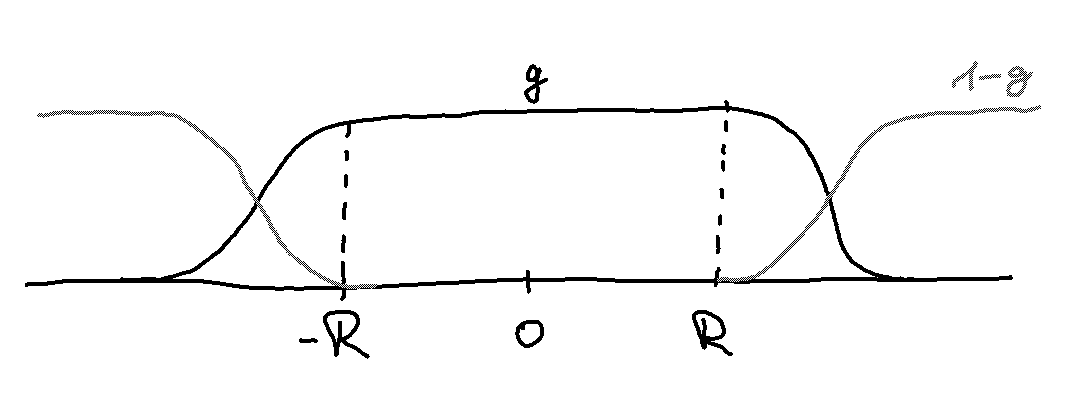
\includegraphics[width=0.75\textwidth]{./pics/Sketch7.png}
			\caption{Skizze der Funktion $g$ und der Funktion $1-g$}
			\label{AbbSkizzeEinsFunktion}
		\end{center}
	\end{figure}
	\underline{Also:} Sei $f\in C_b(\R)$.
	\begin{align*}
		&\left|\int\limits f\d\mu_n-\int\limits f\d\mu\right|\\
		\overset{\text{DU}}{\leq}&
		\underbrace{\Bigg|\int\limits \underbrace{(f\cdot g)}_{\in C_\infty(\R)}-\d\mu_n-\int\limits\underbrace{(f\cdot g)}_{\in C_\infty(\R)}\d\mu\Bigg|}_{\overset{n\to\infty}{\longrightarrow}0\text{ wg. Teil 1}}
		+\left|\int\limits f\cdot(1-g)\d\mu_n-\int\limits f\cdot(1- g)\d\mu_n\right|\\
		\leq&\left|\int\limits (f\cdot g)\d\mu_n-\int\limits(f\cdot g)\d\mu\right|
		+\Vert f\Vert_\infty\cdot\underbrace{\left(\int\limits(1-g)\d\mu_n+\int\limits(1-g)\d\mu\right)}_{
			\begin{subarray}{l}
				\leq\mu_n\big(\R\setminus[-R,R]\big)+\mu\big(\R\setminus[-R,R]\big)\\
				\leq 2\cdot\varepsilon\text{ wegen Straffheit}
			\end{subarray}
		}
	\end{align*}
	\begin{align*}
		&\implies\limn\left|\int\limits f\d\mu_n-\int\limits f\d\mu\right|\leq 2\cdot\varepsilon \mit \varepsilon>0 \text{ beliebig}\\
		&\implies\limn\int\limits f\d\mu_n=\int\limits f\d\mu\qquad\forall f\in C_b(\R)\\
		&\implies\mu_n\overset{\w}{\longrightarrow}\mu
	\end{align*}
\end{proof}

